\begin{usecase}{04}{Dettaglio del regolatore semaforico}
\usecaseprimaryactors{Utente autenticato}
\usecasepre{L'utente sta visionando la lista dei dispositivi collegati al proprio profilo e seleziona un regolatore semaforico dalla lista.}
\usecasedesc{Vengono visualizzati informazioni dettagliate sullo stato del regolatore semaforico.}
\usecasepost{Vengono visualizzati informazioni dettagliate sullo stato del regolatore semaforico.}
\label{uc:UC04}
\end{usecase}

\begin{figure}[!h] 
    \centering 
    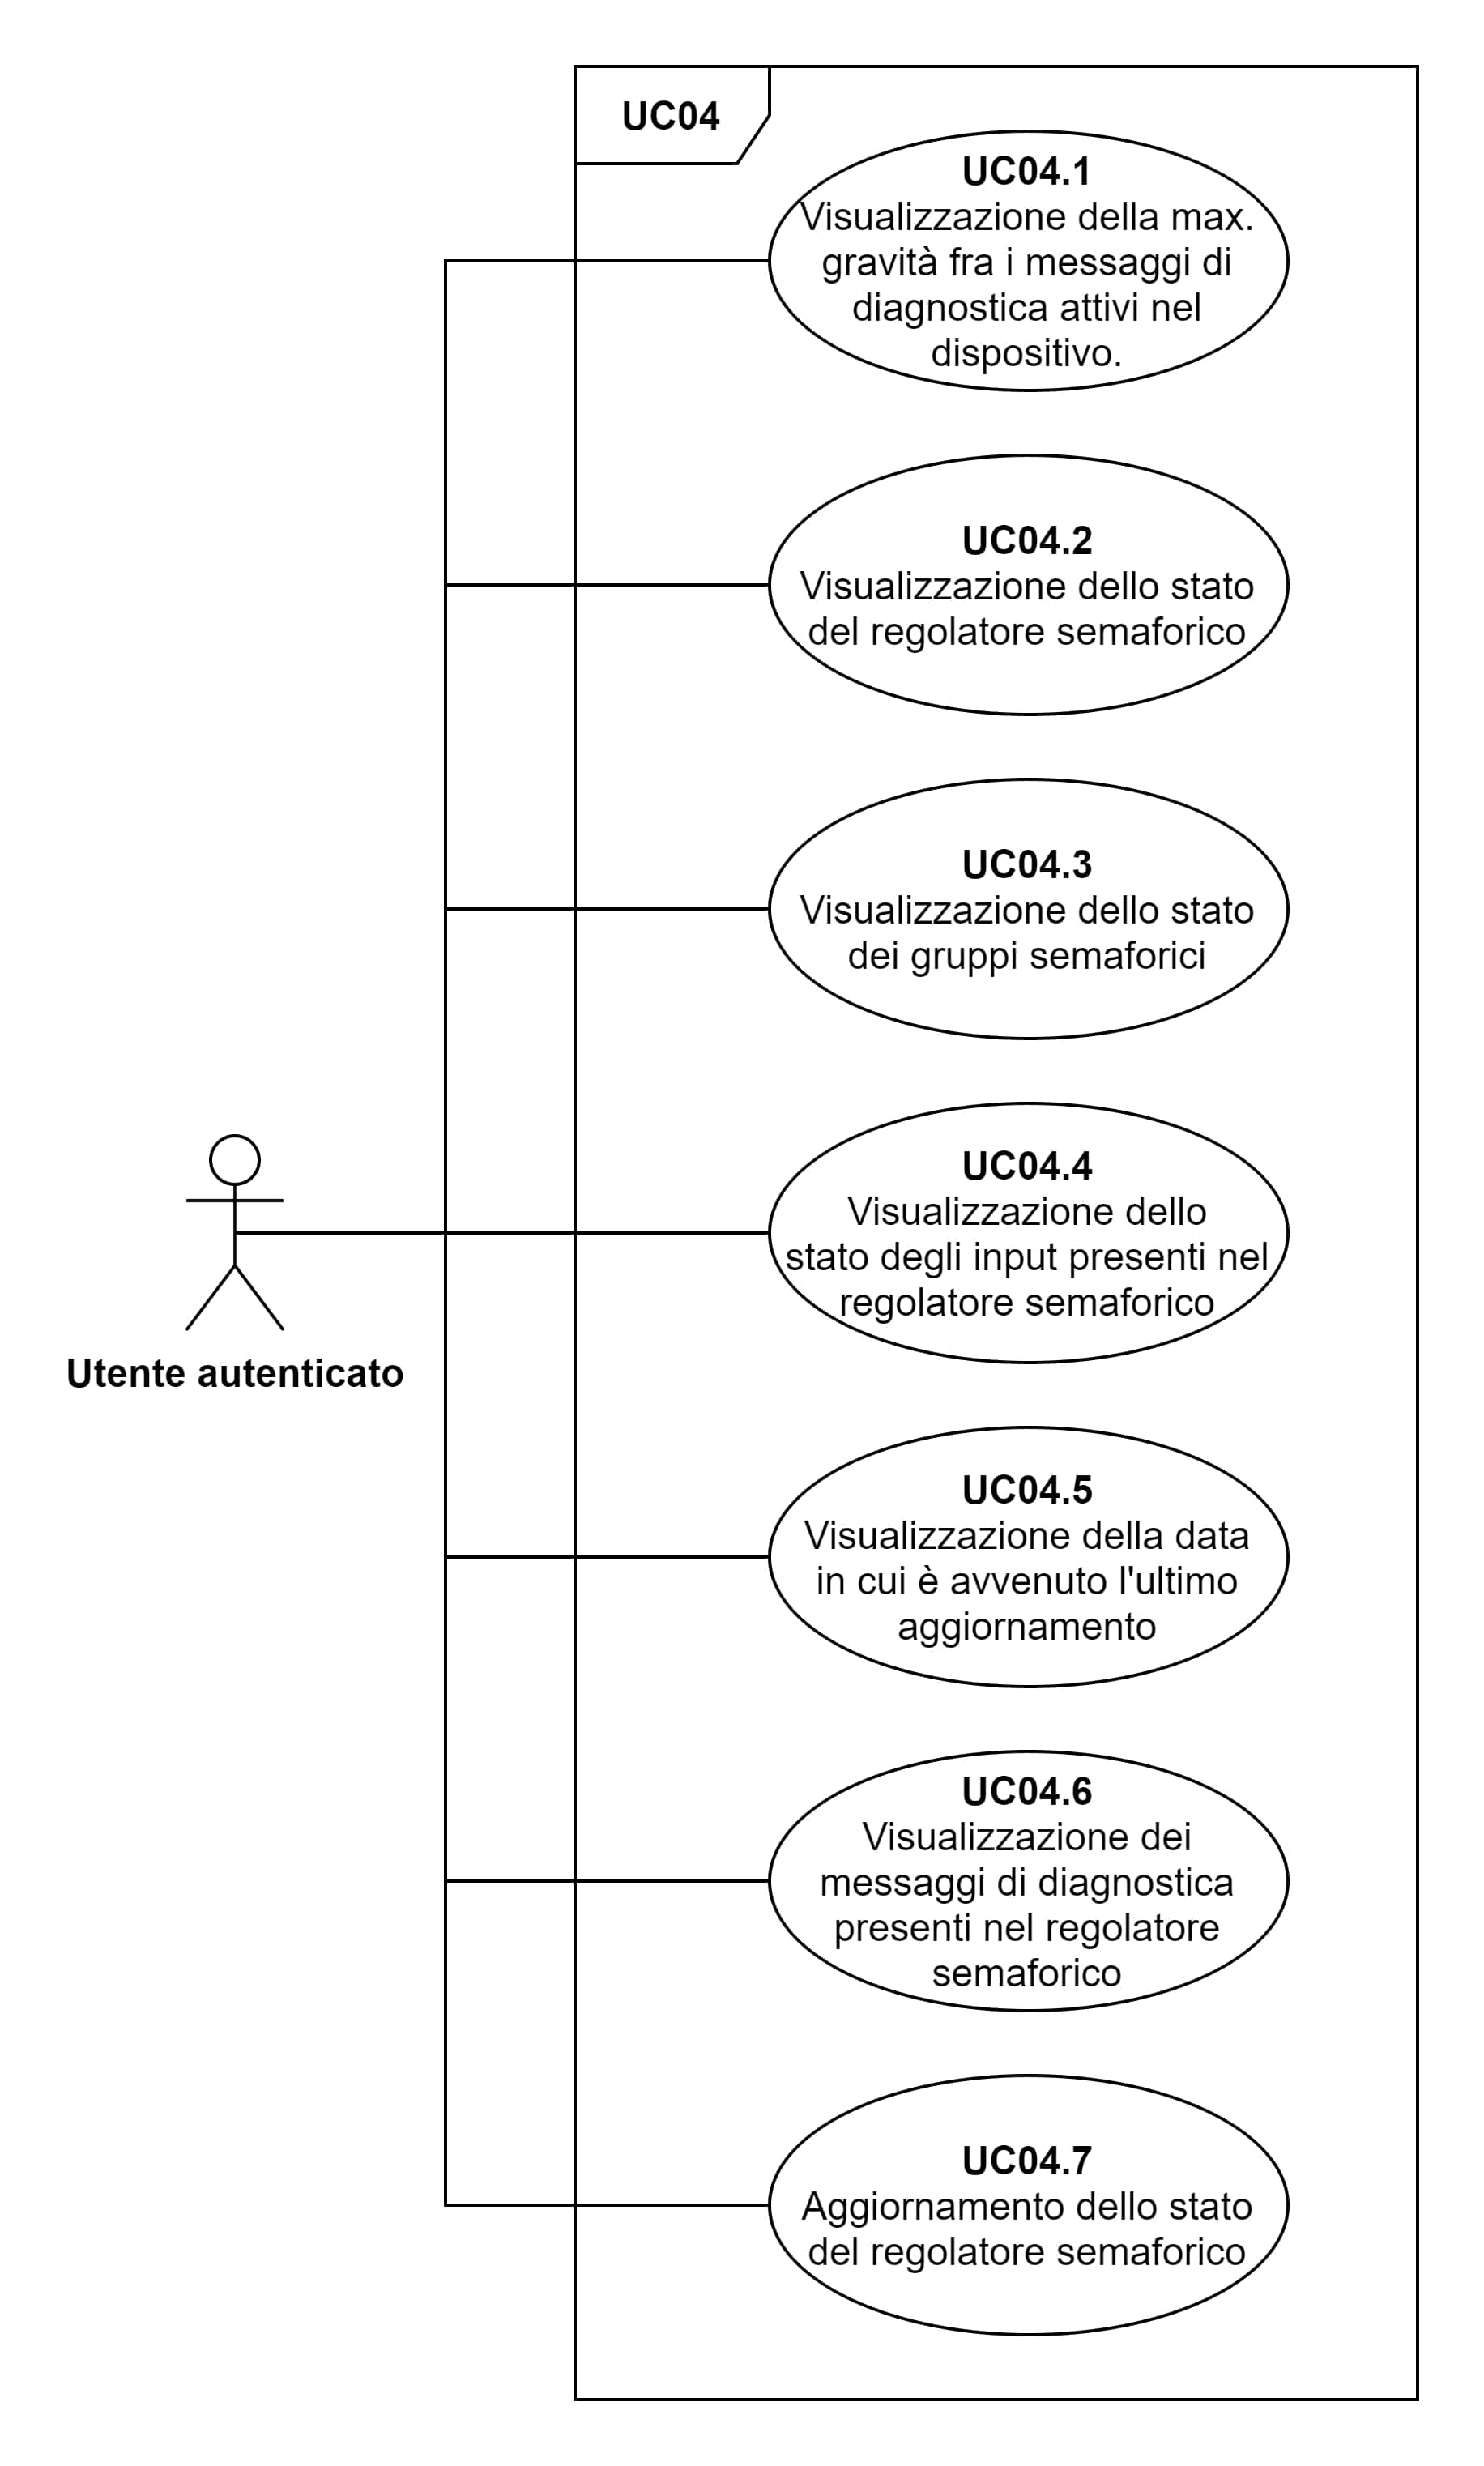
\includegraphics[width=0.9\columnwidth]{appendice-A/uc04} 
    \caption{SMacs - Sotto-casi d'uso di UC04 - Dettaglio del regolatore semaforico}
\end{figure}

\begin{usecase}{04.1}{Visualizzazione della massima gravità fra i messaggi di diagnostica attivi nel dispositivo.}
\usecaseprimaryactors{Utente autenticato}
\usecasepre{L'utente sta visionando il dettaglio del regolatore semaforico selezionato dalla lista.}
\usecasedesc{Viene visualizzato lo stato di diagnostica del regolatore semaforico.}
\usecasepost{Viene visualizzato lo stato di diagnostica del regolatore semaforico.}
\label{uc:UC04-1}
\end{usecase}

\begin{usecase}{04.2}{Visualizzazione dello stato del regolatore semaforico}
\usecaseprimaryactors{Utente autenticato}
\usecasepre{L'utente sta visionando il dettaglio del regolatore semaforico selezionato dalla lista.}
\usecasedesc{Viene visualizzato lo stato del regolatore semaforico (funzione, modalità, livello, step, tempo).}
\usecasepost{Viene visualizzato lo stato del regolatore semaforico (funzione, modalità, livello, step, tempo).}
\label{uc:UC04-2}
\end{usecase}

\begin{usecase}{04.3}{Visualizzazione dello stato dei gruppi semaforici}
\usecaseprimaryactors{Utente autenticato}
\usecasepre{L'utente sta visionando il dettaglio del regolatore semaforico selezionato dalla lista.}
\usecasedesc{Viene visualizzato lo stato dei gruppi semaforici.}
\usecasepost{Viene visualizzato lo stato dei gruppi semaforici.}
\label{uc:UC04-3}
\end{usecase}

\begin{usecase}{04.4}{Visualizzazione dello stato degli input presenti nel regolatore semaforico}
\usecaseprimaryactors{Utente autenticato}
\usecasepre{L'utente sta visionando il dettaglio del regolatore semaforico selezionato dalla lista.}
\usecasedesc{Viene visualizzato lo stato degli input presenti nel regolatore semaforico.}
\usecasepost{Viene visualizzato lo stato degli input presenti nel regolatore semaforico.}
\label{uc:UC04-4}
\end{usecase}

\begin{usecase}{04.5}{Visualizzazione della data in cui è avvenuto l'ultimo aggiornamento}
\usecaseprimaryactors{Utente autenticato}
\usecasepre{L'utente sta visionando il dettaglio del regolatore semaforico selezionato dalla lista.}
\usecasedesc{Viene visualizzata la data dell'ultimo aggiornamento del dettaglio del regolatore semaforico.}
\usecasepost{Viene visualizzata la data dell'ultimo aggiornamento del dettaglio del regolatore semaforico.}
\label{uc:UC04-5}
\end{usecase}

\begin{usecase}{04.6}{Visualizzazione dei messaggi di diagnostica presenti nel regolatore semaforico}
\usecaseprimaryactors{Utente autenticato}
\usecasepre{L'utente sta visionando il dettaglio del regolatore semaforico selezionato dalla lista.}
\usecasedesc{Vengono visualizzati i messaggi di diagnostica presenti nel regolatore semaforico.}
\usecasepost{Vengono visualizzati i messaggi di diagnostica presenti nel regolatore semaforico.}
\label{uc:UC04-6}
\end{usecase}

\begin{usecase}{04.7}{Aggiornamento dello stato del regolatore semaforico}
\usecaseprimaryactors{Utente autenticato}
\usecasepre{L'utente sta visionando il dettaglio del regolatore semaforico selezionato dalla lista.}
\usecasedesc{L'utente seleziona la funzionalità di aggiornamento e viene aggiornato lo stato del regolatore semaforico.}
\usecasepost{L'utente seleziona la funzionalità di aggiornamento e viene aggiornato lo stato del regolatore semaforico.}
\label{uc:UC04-7}
\end{usecase}